% Options for packages loaded elsewhere
\PassOptionsToPackage{unicode}{hyperref}
\PassOptionsToPackage{hyphens}{url}
%
\documentclass[
]{article}
\usepackage{amsmath,amssymb}
\usepackage{lmodern}
\usepackage{iftex}
\ifPDFTeX
  \usepackage[T1]{fontenc}
  \usepackage[utf8]{inputenc}
  \usepackage{textcomp} % provide euro and other symbols
\else % if luatex or xetex
  \usepackage{unicode-math}
  \defaultfontfeatures{Scale=MatchLowercase}
  \defaultfontfeatures[\rmfamily]{Ligatures=TeX,Scale=1}
\fi
% Use upquote if available, for straight quotes in verbatim environments
\IfFileExists{upquote.sty}{\usepackage{upquote}}{}
\IfFileExists{microtype.sty}{% use microtype if available
  \usepackage[]{microtype}
  \UseMicrotypeSet[protrusion]{basicmath} % disable protrusion for tt fonts
}{}
\makeatletter
\@ifundefined{KOMAClassName}{% if non-KOMA class
  \IfFileExists{parskip.sty}{%
    \usepackage{parskip}
  }{% else
    \setlength{\parindent}{0pt}
    \setlength{\parskip}{6pt plus 2pt minus 1pt}}
}{% if KOMA class
  \KOMAoptions{parskip=half}}
\makeatother
\usepackage{xcolor}
\IfFileExists{xurl.sty}{\usepackage{xurl}}{} % add URL line breaks if available
\IfFileExists{bookmark.sty}{\usepackage{bookmark}}{\usepackage{hyperref}}
\hypersetup{
  hidelinks,
  pdfcreator={LaTeX via pandoc}}
\urlstyle{same} % disable monospaced font for URLs
\usepackage[margin=1in]{geometry}
\usepackage{longtable,booktabs,array}
\usepackage{calc} % for calculating minipage widths
% Correct order of tables after \paragraph or \subparagraph
\usepackage{etoolbox}
\makeatletter
\patchcmd\longtable{\par}{\if@noskipsec\mbox{}\fi\par}{}{}
\makeatother
% Allow footnotes in longtable head/foot
\IfFileExists{footnotehyper.sty}{\usepackage{footnotehyper}}{\usepackage{footnote}}
\makesavenoteenv{longtable}
\usepackage{graphicx}
\makeatletter
\def\maxwidth{\ifdim\Gin@nat@width>\linewidth\linewidth\else\Gin@nat@width\fi}
\def\maxheight{\ifdim\Gin@nat@height>\textheight\textheight\else\Gin@nat@height\fi}
\makeatother
% Scale images if necessary, so that they will not overflow the page
% margins by default, and it is still possible to overwrite the defaults
% using explicit options in \includegraphics[width, height, ...]{}
\setkeys{Gin}{width=\maxwidth,height=\maxheight,keepaspectratio}
% Set default figure placement to htbp
\makeatletter
\def\fps@figure{htbp}
\makeatother
\setlength{\emergencystretch}{3em} % prevent overfull lines
\providecommand{\tightlist}{%
  \setlength{\itemsep}{0pt}\setlength{\parskip}{0pt}}
\setcounter{secnumdepth}{5}
\ifLuaTeX
  \usepackage{selnolig}  % disable illegal ligatures
\fi
\usepackage[]{biblatex}

\author{}
\date{\vspace{-2.5em}}

\begin{document}

{
\setcounter{tocdepth}{2}
\tableofcontents
}
\hypertarget{stratification}{%
\section{Stratification}\label{stratification}}

After lodgepole pines (Pinus contorta) have been attacked by Mountain Pine Beetle (MPB), they show different stages. The needles of attacked trees wil turn from green over yellow to red within the first 12 months (red-attack). It then takes in between 1-3 years until all needles have fallen to the ground, when the trees remain standing but without needles (grey-attack) \autocite{wulderRemoteSensingSurvey2005}. Depending on the type of stand, according to \textcite{mitchellFallRateLodgepole1998}, dead trees begin to fall after 3 to 5 years and 80 - 90 \% of trees had fallen after 11 years.
This leads to different stages of beetle attack that will be considered in this study. All green-attack trees detected in 2021 nad 2020 are now with high probability in the red-attack stage. Some of the trees that have been detected as red-attack in 2021, will still classify as red-attack and others as grey-attack. A clear distinction based on time of detection is not possible without additional data, since it can take several years before all needles have fallen of the tree, the GPS locations of MPB-attacked trees provided by the government of Alberta \autocite{wulderRemoteSensingSurvey2005}. Collecting the LiDAR data at the end of May, all green-attack trees that have been attacked in 2019 and before, as well as all red-attack trees detected in 2020 and before, will now classify as grey attack. Additionally, it can be expected that most of the trees that have been detected as red-attack in 2011 and before, now have fallen to the ground \autocite{schoennagelEffectsMountainPine2012}.

Three broad areas of interest have been selected (refer to fig AoIs) based on availability of observed MPB attacks in the years 2011, 2019, 2020, and 2021, while also having a dense network of paved roads and gravel roads. These areas of interest will be referred to as th Grande Prairie (GP) area in the North-West, the Whitecourt (WC) area in the North-East, and the Rocky Mountain House (RMH) area to the South-East.

\begin{figure}

{\centering 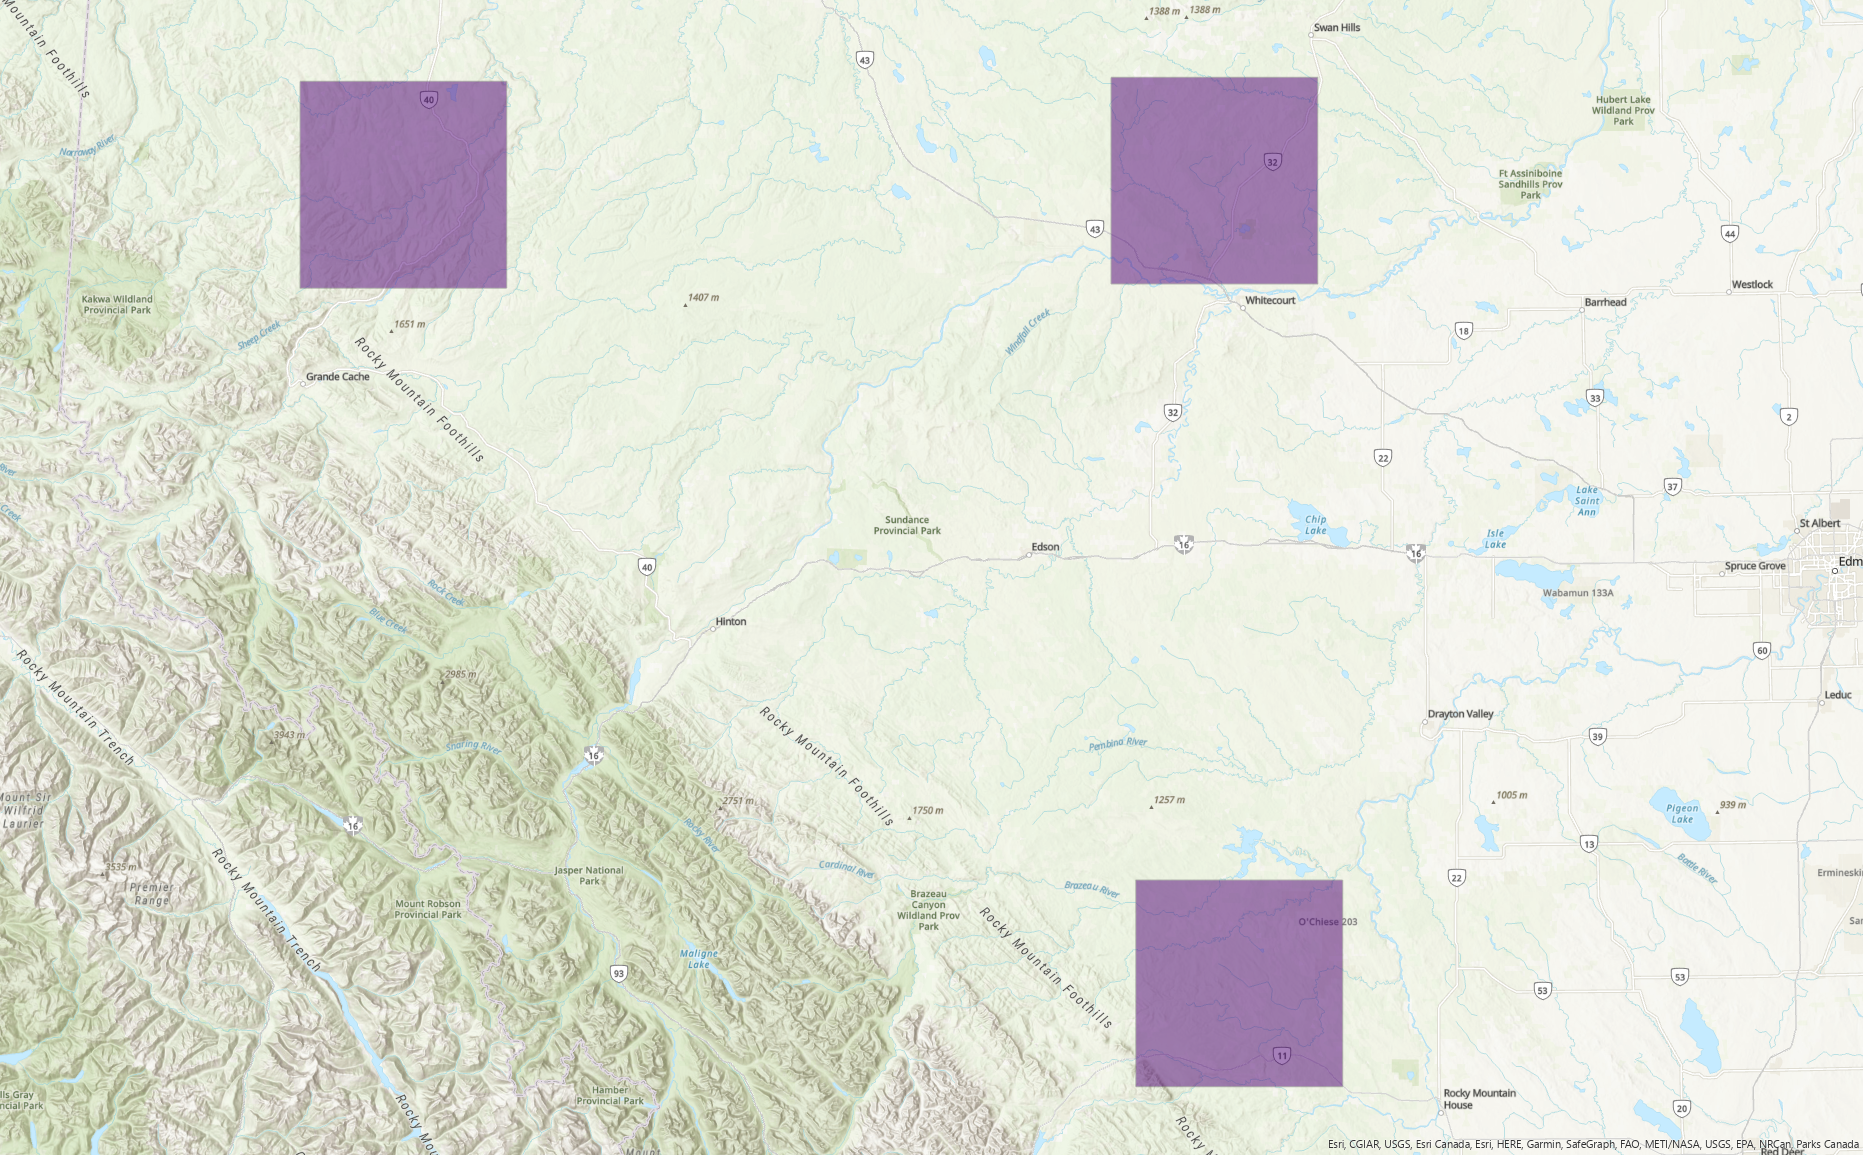
\includegraphics[width=0.8\linewidth]{../graphics/AreasOfInterest} 

}

\caption{50 km by 50 km areas of interest for further investigation.}\label{fig:AoIs}
\end{figure}

As already shown by various authors before, lodgepole pine (Pinus contorta) is the most commonly attacked by MPB, thus, areas where chosen, where lodgepole pine is one of the most dominant species. This information was based on a visual analysis of species classification, how it was in 2019, on a 30 m by 30 m grid. Each resulting pixel is classified as the most dominant tree species within that pixel. Where trees were not the dominant species, the pixel is classified as ``No Tree''. Table \ref{tab:species} shows all species that dominate the area classified within at least one pixel and their corresponding value and NFI codes.

\begin{table}

\caption{\label{tab:species}Value and NFI Code for Species Common Names}
\centering
\begin{tabular}[t]{lccc}
\toprule
Value Code & NFI Code & Common Species Name & Scientific Species Name\\
\midrule
0 & NO.TREE & No Trees & \\
2 & ABIE.BAL & Balsam Fir & Abies balsamea\\
3 & ABIE.LAS & Subalpine Fir & Abies lasiocarpa\\
10 & BETU.PAP & White Birch & Betula papyrifera\\
13 & LARI.LAR & Tamarack & Larix laricina\\
\addlinespace
16 & PICE.ENG & Engelmann Spruce & Picea engelmannii\\
17 & PICE.GLA & White Spruce & Picea glauca\\
18 & PICE.MAR & Black Spruce & Picea mariana\\
22 & PINU.BAN & Jack Pine & Pinus banksiana\\
23 & PINU.CON & Lodgepole Pine & Pinus contorta\\
\addlinespace
27 & POPU.BAL & Balsam Poplar & Populus balsamifera\\
29 & POPU.TRE & Trembling Aspen & Populus tremuloides\\
30 & PSEU.MEN & Douglas-Fir & Pseudotsuga menziesii\\
35 & TSUG.HET & Western Hemlock & Tsuga heterophylla\\
\bottomrule
\end{tabular}
\end{table}

The government of Alberta conducts annual Heli-GPS surveys, usually between August 15 and September 15 by flying helicopters at low hight and mapping the GPS locations of detected disturbances in therms of red- and green-attack through observers. These locations have a positional accuracy of +/- 30 m. In most cases only patches consisting of at least 3 trees are recorded. For each of these locations the corresponding cell from the raster data containing the tree species is determined and with a box filter of 5 by 5 the most common tree species for each point can be determined. An example for these buffered GPS locations and the corresponding species data is shown in fig.~\ref{fig:bufferedPointsExample}. This analysis is performed for each of the three areas of interest, both in absolute numbers of pixels within each kernel and relative to the total number of included pixels for each year. It is possible that an area surrounding a GPS location only consists of pixels that have been classified as ``No Tree''. This only means that, in 2019 when the data had been collected, the corresponding 30 by 30 m cell was not predominantlyS covered by trees.

\begin{figure}

{\centering 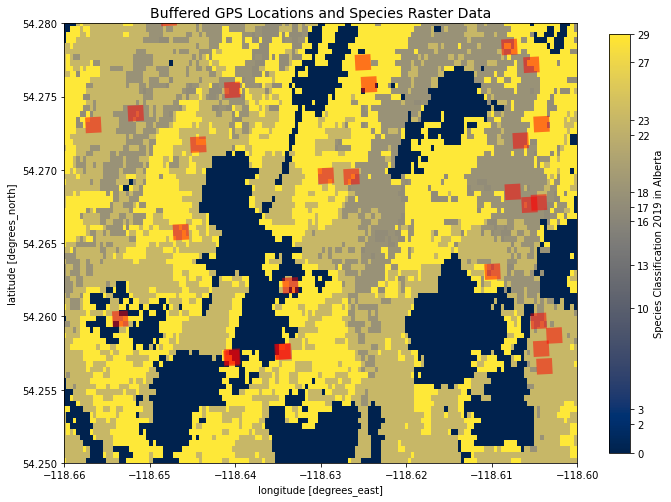
\includegraphics[width=0.8\linewidth]{../graphics/bufferedPointsExample} 

}

\caption{Exemplary buffered GPS locations}\label{fig:bufferedPointsExample}
\end{figure}
\begin{figure}

{\centering 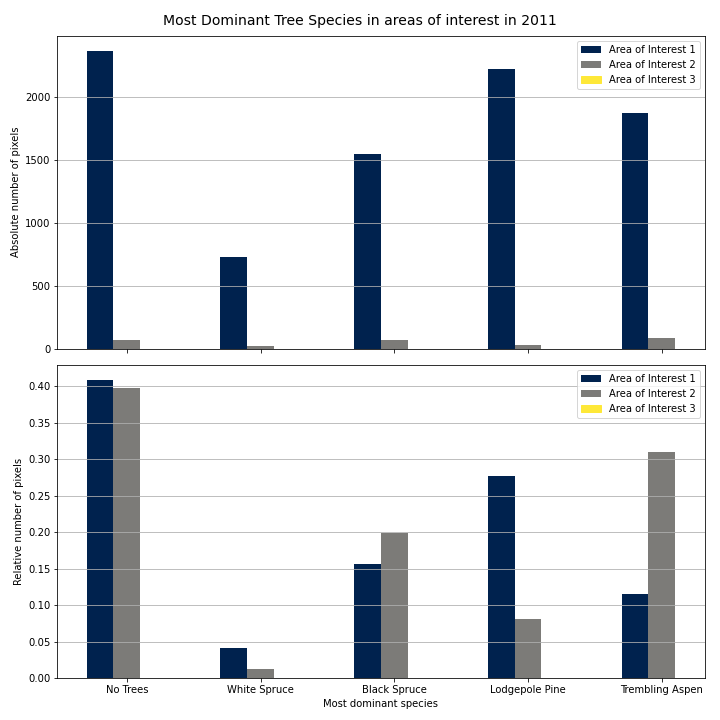
\includegraphics[width=0.8\linewidth]{../graphics/freq_species_11} 

}

\caption{Frequency of tree species within the surrounding area of each MPB survey point for the year 2011.}\label{fig:freqSpecies11}
\end{figure}
\begin{figure}

{\centering 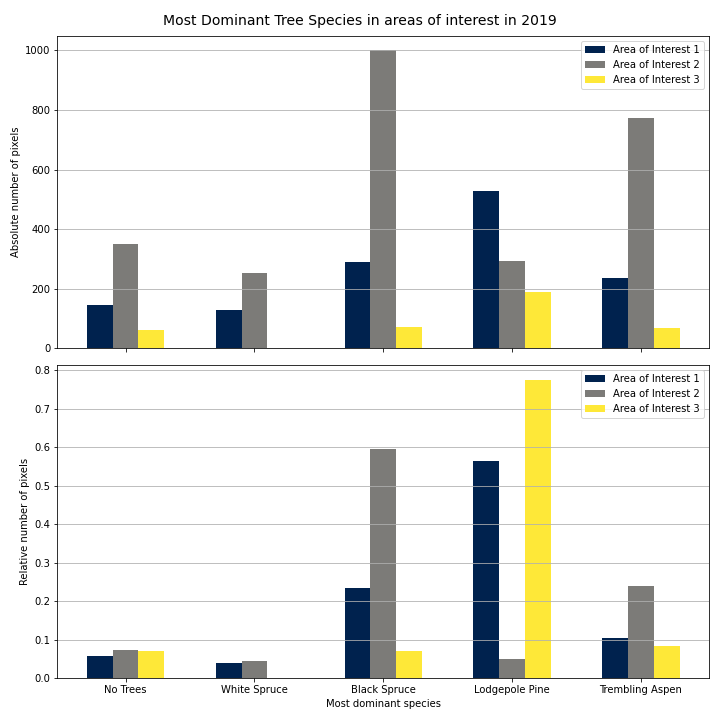
\includegraphics[width=0.8\linewidth]{../graphics/freq_species_19} 

}

\caption{Frequency of tree species within the surrounding area of each MPB survey point for the year 2011.}\label{fig:freqSpecies19}
\end{figure}
\begin{figure}

{\centering 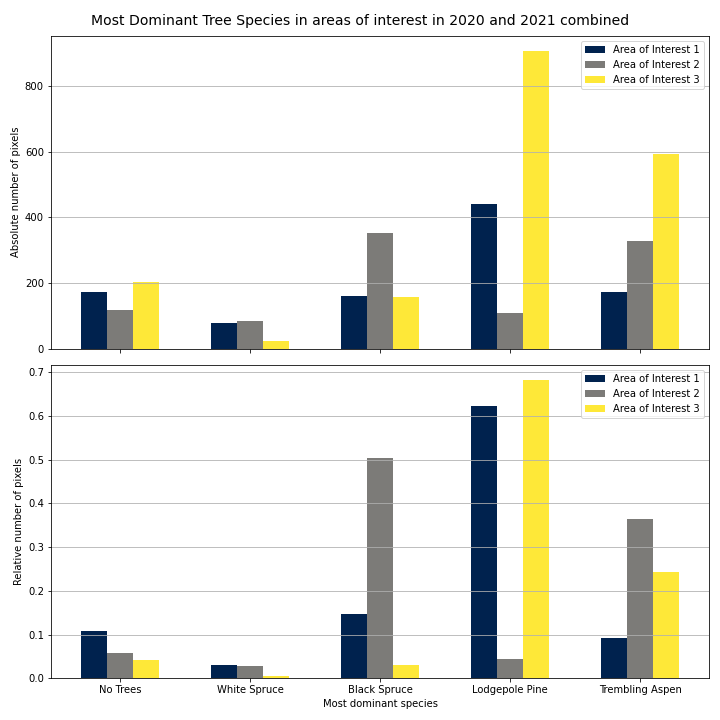
\includegraphics[width=0.8\linewidth]{../graphics/freq_species_20_21} 

}

\caption{Frequency of tree species within the surrounding area of each MPB survey point for the year 2011.}\label{fig:freqSpecies20-21}
\end{figure}

Information on accessibility is based on the road network available through the government of Alberta \autocite{GravelRoad2021,PavedRoad2021}, since all flight locations with the drone need to be accessible from the road for efficient data collection. As the drone has to stay in line of sight, it is not possible to fly far away from the road.

This document was written with bookdown \autocite{R-bookdown}.

\hypertarget{references}{%
\section{References}\label{references}}

\hypertarget{references}{}

\printbibliography

\end{document}
